\chapter{Resonance Decays}

\section{Decay Map and Energy Conservation}

If the particles considered on the freezout surface are not stable, the spectra computed there cannot be directly related to the spectra on the detector surface. Instead, one has to calculate contributions from all possible decay channels/heavier resonances $a$ that decay into the (stable) resonance $b$ under consideration. This is done via the linear decay map
\begin{equation}
    E_{\vec{p}}\frac{\dt N_b}{\dt^3p}=\int\frac{\dt^3q}{(2\pi)^3}\frac{1}{2\omega_{\vec{p}}}D^a_b(\vec{p},\vec{q})E_{\vec{q}}\frac{\dt N_a}{\dt^3 q}
\end{equation} 
where $D_{a\rightarrow b}(\vec{p},\vec{q})$ is the Lorentz invariant probability of particle $a$ with (on-shell) momentum $\vec{q}$ to decay into particle $b$ with momentum $\vec{p}$. Due to the probabilistic nature of a decay process, this relation is true if the lifetime of the heavy resonances is short compared to the propagation time and the number of particles is large enough.

Assuming isotropic decay, a two-body decay $a\rightarrow b+c$ is modelled by the decay map 
\begin{equation}
    D^a_{b\vert c}(\vec{p},\vec{q})=D^a_{b\vert c}(p^\mu q_\mu)=B\frac{4\pi^2 m_a}{p^a_{b\vert c}}\delta(q^\mu p_\mu+m_a E^a_{b\vert c})
\end{equation}
where $B$ is the branching ratio of the decay and
\begin{equation}
    p^a_{b\vert c}=\frac{1}{2m_a}\sqrt{\big((m_a+m_b)^2-m_c^2\big)\big((m_a-m_b)^2-m_c^2\big)}\,,\qquad E^a_{b\vert c}=\sqrt{m_b^2+(p^a_{b\vert c})^2}\,.
\end{equation}
In the rest frame of particle $a$ one finds $\vec{p}\equiv \vec{p}_b=-\vec{p}_c$, energy conservation is expressed as
\begin{equation}
    m_a=\sqrt{m_b^2+\vec{p}^2}+\sqrt{m_c^2+\vec{p}^2}
\end{equation}
with the solution space restricted only by $\vec{p}^2=(p^a_{b\vert c})^2$. The energy of particle $b$ in the rest frame of $a$, expressed covariantly, is just $E^a_{b\vert c}=-\frac{1}{m_a}q^\mu p_\mu$ and thus the above formula simply represents energy conservation.

To decompose the above energy conserving delta function, rewrite $q^\mu p_\mu$ in the coordinates used in \ref{sec:SpectraCoordinateSystem}.
\begin{equation}
    q^\mu p_\mu=-m_{q,T} m_{p,T}\cosh(\eta_q-\eta_p)+q_T p_T\cos(\varphi_q-\varphi_p)
\end{equation}
We shall resolve the $\delta$-distribution using the identity
\begin{equation}
    \int\dt^dx f(x^i)\delta(g(x^i))=\int_{g^{-1}(0)}\dt^{d-1}\sigma\frac{f(x^i)}{\Vert\vec{\nabla}g(x^i)\Vert}\,,
\end{equation}
interchanging a $\delta$-distribution of a multivariate function $g$ for an integration over the codimension-1 hypersurface formed by the level set ${g^{-1}(0)}$, considering the induced metric and further warping factors from the gradient, that seem intuitive from the ${(d=1)}$-case of this identity.

In detail, we use rotational and boost symmetry to eliminate the $\varphi_p$ and $\eta_p$ dependence and apply the variable changes
\begin{gather*}
    \int_0^\infty\dt\eta\;f(\cosh\eta)=\int_1^\infty\dt u\frac{f(u)}{\sqrt{u^2-1}}\,,\qquad \int_0^\pi\dt\varphi\;f(\cos\varphi)=\int_{-1}^1\dt v\frac{f(v)}{\sqrt{1-v^2}}\\
   \text{and}\qquad q_T=Q t\quad\text{with}\;Q=\const\;\text{and}\;[Q]=\text{GeV}\,,\;[t]=1\,.
\end{gather*}
(omit the $\tilde{\cdot}$ in the following) and defined $u^\star(t,v)$ to respect the $\delta$. The $\delta$-distribution depending on the variables ${(t,u,v)}$ and the parameters ${(Q,p_T)}$ was replaced by considering the function
\begin{equation}
    g(t,u,v)=-u\,\omega_{q,T} \omega_{p,T} +t\,v\,Qp_T+m_a E^a_{b\vert c}\,,\quad
        \vec{\nabla} g=
        \begin{pmatrix}
            -t\,u\,Q^2\frac{\omega_{p,T}}{\omega_{q,T}}+v\,Q p_T\\
            -\omega_{q,T}\omega_{p,T}\\
            t\,Q p_T
        \end{pmatrix}\,.
\end{equation}
% \begin{subequations}
%     \begin{align}
%         g(t,u,v)&=-u\omega_{q,T} \omega_{p,T} +tvQ p_T+m_a E^a_{b\vert c}\\
%         \vec{\nabla} g&=
%         \begin{pmatrix}
%             -t\,u\,\frac{\omega_{p,T}}{\omega_{q,T}}Q^2+vQ p_T\\
%             -\omega_{q,T}\omega_{p,T}\\
%             t\,Q p_T
%         \end{pmatrix}\,.
%     \end{align}
% \end{subequations}
The manifold defined by the level set where ${g(t,u,v)=0}$ is given by 
\begin{equation}
    g^{-1}(0)=\Bigg\{(t,u,v)\Big\vert u=u^\star(t,v)=\frac{m_a E^a_{b\vert c}+t\,v\,Q p_T}{\omega_{q,T}\omega_{p,T}}\Bigg\}\,.
    \label{eq:DecayMap_BjorkenCoord_DeltaManifold}
\end{equation}
Equation \eqref{eq:DecayMap_BjorkenCoord_DeltaManifold} defines a chart $(t,v)\mapsto x^i(t,v)=(t,u^\star(t,v),v)$ on $g^{-1}(0)$ with coordinates $(t,v)$. One computes the coordinate derivative vectors and oriented surface element
\begin{gather}
    \frac{\partial x^i}{\partial t}
        % =\begin{pmatrix}
        %     1\\
        %     \frac{v\,Qp_T}{\omega_{p,T}\omega_{q,T}}-\frac{t\,Q^2(m_a E^a_{b\vert c}+t\,v\,Q p_T)}{\omega_{p,T}(\omega_{q,T})^3}\\
        %     0
        % \end{pmatrix}
        =\begin{pmatrix}
            1\\
            \frac{m_aQ(-t\,QE^a_{b\vert c}+v\,m_a p_T)}{\omega_{p,T}(\omega_{q,T})^3}\\
            0
        \end{pmatrix}\,,\quad
    \frac{\partial x^i}{\partial v}=\begin{pmatrix}
        0\\
        \frac{t\,Qp_T}{\omega_{p,T}\omega_{q,T}}\\
        1
    \end{pmatrix}\,,\\
    \dt\Sigma^i=\frac{\partial x^i}{\partial t}\times \frac{\partial x^i}{\partial v}\dt t\dt v=\begin{pmatrix}
        \frac{m_aQ(-t\,QE^a_{b\vert c}+v\,m_a p_T)}{\omega_{p,T}(\omega_{q,T})^3}\\
        -1\\
        \frac{t\,Qp_T}{\omega_{p,T}\omega_{q,T}}
    \end{pmatrix}\dt t\dt v\,.
\end{gather}
which defines the scalar surface element via $\dt^2\sigma=\sigma(t,v)\dt t\dt v=\Vert\dt\Sigma^i\Vert$. The result of this calculation (see Appendix \ref{sec:Apdx_ResonanceComput}) is given by
\begin{multline}
    \omega_{\vec{p}}\frac{\dt N_b}{\dt^3p}=\frac{BQ^2}{\pi p^a_{b\vert c}}\int_0^\infty\dt t\int_{-1}^1\dt v\;t\;\Big(\omega_{\vec{q}}\frac{\dt N_a}{\dt^3 q}\Big)\Big\vert_{t\cdot Q }\times\\
    \times\Bigg(\frac{\Theta(u-1)}{\sqrt{u^2-1}}\frac{1}{\sqrt{1-v^2}}\frac{\sigma(t,v)}{\Vert\vec{\nabla}g(t,u,v)\Vert}\Bigg)\Bigg\vert_{u=u^\star(t,v)}\,.
    \label{eq:DecayCalc_FinalIntegral}
\end{multline}

\paragraph{Restricting the Integration Domain}

For the numerics, the integration interval of $t$ can be kept finite for 2 reasons. First, the spectrum of the primary resonance can be assumed to decay sufficiently fast. Second, not all combinations ${(t,v)}$ correspond to physically allowed momenta for the decay process. To see this, note that ${\lim_{t\to\infty}u^\star(t,v)<1}$ for every finite value of $p_T$. Since by definition ${u=\cosh\eta>0}$, there are no contributions to the integral at large $t$. Actually, the restriction ${u^\star(t,v)\geq 1}$ allows for drastic reduction of the integration domain in both $t$- and $v$-direction, which is especially important for the seemingly divergent - nevertheless integrable - integrand. This is ultimately a consequence of energy conservation, allowing only for specific values of momentum rapidity, encoded by $u$.

It is instructive to see how this restriction looks like in formula. A priori, the integration domain is the partially unbounded rectangular region ${\{(t,v)\in[0,\infty]\times[-1,1]\}}$. The line ${u^\star(t,v)=1}$ separates this domain into 2 regions, only 1 of which contributes to the above integration, namely where ${u^*(t,v)>1}$. In the $t-v$-plane, this line is given as a function ${v_1(t)}$ by
\begin{equation}
    v_1(t)=\frac{\omega_{T,p}\omega_{T,q}-m_aE^a_{b\vert c}}{t\,Qp_T}\,.
    \label{eq:DecayCalc_v1t}
\end{equation}
If we were to perform the multidimensional integration ${\iint\dt t\dt v}$ via nested integrals, this would be sufficient, since we could first perform the $v$-integration over a $t$-dependent range and then integrate over $t$. Unfortunately this performs very poorly on the numeric side due to the iterative subdivision of the exterior integral causing a very large number of numerical evaluations of the interior integral. Instead, efficient multidimensional integration requires us to subdivide the $n$-dimensional integration domain in rectangular subdomains, thus looking for the smallest possible rectangular integration domain is desirable. This is the idea of cubature algorithms.

To do so, we want to find the minimal and maximal values of $t$ and $v$. By definition ${v=\cos\varphi}$ and it is clear that ${v_{\text{max}}=1}$ by noting that ${\lim_{t\to\infty}v_1(t)>1}$. It is also clear that ${u^\star(t,v)>1}$ only if ${v>v_1(t)}$. Thus, in order to find a minimum value of $v$, we need to find the minimum of $v_1(t)$, which is located at
\begin{equation}
    t^\prime=\frac{m_a\sqrt{(\omega_{p,T})^2-(E^a_{b\vert c})^2}}{QE^a_{b\vert c}}\,,\qquad v_{\text{min}}=v_1(t^\prime)=\frac{\sqrt{(\omega_{p,T})^2-(E^a_{b\vert c})^2}}{p}\,.
    \label{eq:Cubature_vmin}
\end{equation}
This minimum only exists when ${\omega_{p,T}>E^a_{b\vert c}}$ or equivalently ${p_T>p^a_{b\vert c}}$. In this case, not only ${\lim_{t\to\infty}v_1(t)>1}$, but also ${\lim_{t\to0}v_1(t)>1}$. Therefore, minimal and maximal values of $t$ can be determined via
\begin{equation}
    v_1(t_{\text{max/min}})=1\qquad\iff\qquad t_{\text{max/min}}=\frac{m_a\big(p_TE^a_{b\vert c}\pm p^a_{b\vert c}\omega_{p,T}\big)}{m_b^2Q}\,.
    \label{eq:Cubature_tminmax}
\end{equation}
On the other hand, if ${\omega_{p,T}<E^a_{b\vert c}}$, it is obvious that ${\lim_{t\to0}v_1(t)=-\infty}$, and therefore one sets ${v_{\text{min}}=-1}$ and accordingly ${t_{\text{min}}=0}$.

To summarize, the smallest rectangular regions ${[t_{\text{min}},t_{\text{max}}]\times[v_{\text{min}},v_{\text{max}}]}$ are given by
\debugbox{
    \begin{minipage}{\linewidth}  
        \centering      
        \begin{tabular}{ c 
            !{\vrule width 2pt}c 
            !{\vrule width 1pt}c 
            !{\vrule width 1pt}c 
            !{\vrule width 1pt}c}
            &$t_{\text{min}}$&$t_{\text{max}}$&$v_{\text{min}}$&$v_{\text{max}}$\\
            \noalign{\hrule height 2pt}
            ${\omega_{p,T}<E^a_{b\vert c}}$&$0$&\eqref{eq:Cubature_tminmax}&$-1$&$1$\\
            \noalign{\hrule height 1pt}
            ${\omega_{p,T}>E^a_{b\vert c}}$&\eqref{eq:Cubature_tminmax}&\eqref{eq:Cubature_tminmax}&\eqref{eq:Cubature_vmin}&$1$
        \end{tabular}
        \captionof{table}{Smallest rectangular regions ${[t_{\text{min}},t_{\text{max}}]\times[v_{\text{min}},v_{\text{max}}]}$ that contain the entire relevant integration domain for the decay computation.}
    \end{minipage}
}
Obviously, the integration domain becomes drastically smaller as soon as ${\omega_{p,T}>E^a_{b\vert c}}$. This is the threshold where the unstable heavy particle $a$ cannot be at rest (${q_T=0}$) in order to decay into a lighter particle $b$ with possibly large momentum ${p_T>0}$. Above this threshold, the possible values of ${v\geq v_{\text{min}}}$ get closer to $1$, meaning the momenta of heavy resonance and decay product become increasingly aligned. The above considerations are summarized graphically in\\\noindent
\debugbox{
    \begin{minipage}{\linewidth}
        \centering
        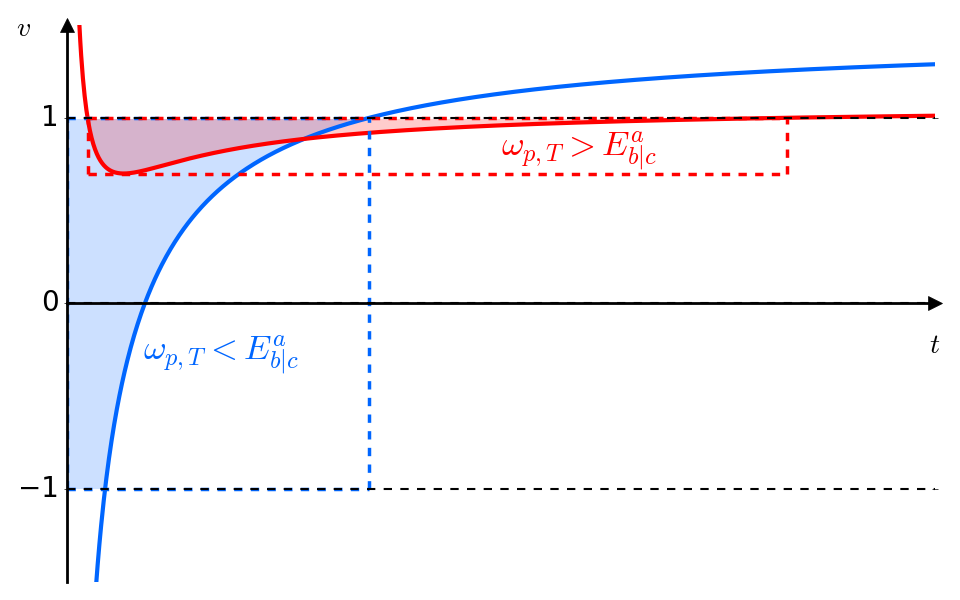
\includegraphics[width=0.8\linewidth]{code/C++/DCCspec/otherfiles/DecayCalc_IntegrDom.png}
        \captionof{figure}{Depiction of the integration domain for the 2 cases ${\omega_{p,T}<E^a_{b\vert c}}$ (blue) and ${\omega_{p,T}>E^a_{b\vert c}}$ (red). Solid lines show the graph of ${v_1(t)}$ (see equation \eqref{eq:DecayCalc_v1t}), the shaded regions are the regions of non-vanishing contributions in the integral \eqref{eq:DecayCalc_FinalIntegral}, i.e. the relevant integration domain defined by ${u^\star(t,v)\geq 1}$. Dashed lines are the boundaries of the smallest rectangular integration domains in each case.}
        \label{fig:DecayCalc_IntegrDom}
    \end{minipage}
}

% \paragraph*{Again without Change of Variables}\mbox{}\\

% \begin{subequations}
%     \begin{align}
%         \omega_{\vec{p}}\frac{\dt N_b}{\dt^3p}&=B\frac{4\pi^2m_a}{p^a_{b\vert c}}\times2\pi\int\frac{\dt^4q}{(2\pi)^4}\delta(q^2+m^2)\omega_{\vec{q}}\frac{\dt N_a}{\dt^3 q}\delta\big(q^\mu p_\mu+m_a E^a_{b\vert c}\big)\\
%         &=B\frac{4\pi^2m_a}{p^a_{b\vert c}}\times2\pi\int_{(0,0,-\infty,0)}^{(\infty,\infty,\infty,2\pi)}\frac{\dt m_{q,T} \dt Q\dt\eta_q\dt\varphi_q}{(2\pi)^4}m_{q,T} Q\delta(-m_{q,T}^2+q_T^2+m^2)\omega_{\vec{q}}\frac{\dt N_a}{\dt^3 q}\times\nonumber\\
%         &\phantom{=}\qquad\times\delta\big(-m_{q,T} m_{p,T}\cosh(\eta_q-\eta_p)+Q p_T\cos(\varphi_q-\varphi_p)+m_a E^a_{b\vert c}\big)\\
%         &=B\frac{4\pi^2m_a}{p^a_{b\vert c}}\times2\pi\int_{(0,-\infty,0)}^{(\infty,\infty,2\pi)}\frac{\dt Q\dt\eta_q\dt\varphi_q}{(2\pi)^4}\frac{Q}{2}\omega_{\vec{q}}\frac{\dt N_a}{\dt^3 q}\times\nonumber\\
%         &\phantom{=}\qquad\times\delta\big(-\omega_{q,T} \omega_{p,T}\cosh\eta_q+Q p_T\cos\varphi_q+m_a E^a_{b\vert c}\big)\\
%         &=B\frac{4\pi^2m_a}{p^a_{b\vert c}}\times2\pi\times 2\times 2\int_{(0,0,0)}^{(\infty,\infty,\pi)}\frac{\dt Q\dt\eta_q\dt\varphi_q}{(2\pi)^4}\frac{Q}{2}\omega_{\vec{q}}\frac{\dt N_a}{\dt^3 q}\times\nonumber\\
%         &\phantom{=}\qquad\times\delta\big(-\omega_{q,T} \omega_{p,T}\cosh\eta_q+Q p_T\cos\varphi_q+m_a E^a_{b\vert c}\big)\\
%         \intertext{\dots using $Q\mapsto t\cdot Q$, where $Q=\const$ carries the dimension and $t\in[0,\infty)$ is dimensionless, we calculate (omit the $\tilde{\cdot}$)}
%         &=B\frac{4\pi^2m_a}{p^a_{b\vert c}}\times\frac{4\pi Q^2}{(2\pi)^4}\times\int_0^\infty\dt t\int_0^\pi\dt\varphi\cdot t\cdot \Big(\omega_{\vec{q}}\frac{\dt N_a}{\dt^3 q}\Big)\Big\vert_{t\cdot Q}\frac{\sigma(t,\varphi)}{\Vert\vec{\nabla}g(t,\eta^\star,\varphi)\Vert}
%     \end{align}
% \end{subequations}
% Here we defined
% \begin{subequations}
%     \begin{align}
%         g(t,\eta,\varphi)&=-\omega_{q,T} \omega_{p,T} \cosh\eta+Q p_T t\cos\varphi+m_a E^a_{b\vert c}\\
%         \vec{\nabla} g&=
%         \begin{pmatrix}
%             -\frac{\omega_{p,T}}{\omega_{q,T}}Q^2 \cdot t\cdot\cosh\eta+Q p_T \cos\varphi\\
%             -\omega_{q,T}\omega_{p,T}\sinh\eta\\
%             -t\cdot Q p_T\sin\varphi
%         \end{pmatrix}
%     \end{align}
% \end{subequations}
% implying 
% \begin{equation}
%     g^{-1}(0)=\Bigg\{(t,\eta,\varphi)\Big\vert\eta=\eta^\star(t,\varphi)=\arcosh\Big(\underbrace{\frac{m_a E^a_{b\vert c}+t\cdot Q p_T\cos\varphi}{\omega_{q,T}\omega_{p,T}}}_{\eqdef u^\star(t,\varphi)}\Big)\Bigg\}
% \end{equation}
% One this manifold we need the surface element $\sigma(t,\varphi)\dt t\dt\varphi$. For some $x^i\in g^{-1}(0)$ the coordinate derivatives and surface normal are given by
% \begin{subequations}
%     \begin{align}        
%         \frac{\partial x^i}{\partial t}=\begin{pmatrix}
%             1\\
%             \frac{1}{\sqrt{(u^\star)^2-1}}\frac{\partial u^\star}{\partial t}\\
%             0
%         \end{pmatrix}&=\begin{pmatrix}
%             1\\
%         \frac{1}{\sqrt{(u^\star)^2-1}}\cdot\frac{Q p_T}{\omega_{q,T}\omega_{p,T}}\cos\varphi\Big(1-t^2\big(\frac{Q}{\omega_{q,T}}\big)^2\Big)\\
%         0
%     \end{pmatrix}\\
%     \frac{\partial x^i}{\partial \varphi}=\begin{pmatrix}
%         0\\
%         \frac{1}{\sqrt{(u^\star)^2-1}}\frac{\partial u^\star}{\partial\varphi}\\
%         1
%     \end{pmatrix}&=\begin{pmatrix}
%         0\\
%         -\frac{1}{\sqrt{(u^\star)^2-1}}\frac{Q p_T}{\omega_{q,T}\omega_{p,T}}\cdot t\sin\varphi\\
%         1
%     \end{pmatrix}\\
%     \dt^2\sigma^i=\frac{\partial x^i}{\partial t}\times\frac{\partial x^i}{\partial\varphi}\dt t\dt\varphi&=\begin{pmatrix}
%         \frac{1}{\sqrt{(u^\star)^2-1}}\cdot\frac{Q p_T}{\omega_{q,T}\omega_{p,T}}\cos\varphi\Big(1-t^2\big(\frac{Q}{\omega_{q,T}}\big)^2\Big)\\
%         -1\\
%         -\frac{1}{\sqrt{(u^\star)^2-1}}\frac{Q p_T}{\omega_{q,T}\omega_{p,T}}\cdot t\sin\varphi
%     \end{pmatrix}\dt t\dt\varphi\\
%     \sigma(t,\varphi)\dt t\dt\varphi&\defeq \Vert\dt^2\sigma^i\Vert
% \end{align}
% \end{subequations}

\section{Decay Spectra}

Moving toward some results and actual spectra, let us try to investigate the decay ${a\to b+b}$ of a heavy particle $a$ into 2 equal lighter particles $b$. This is effectively the situation to be considered for the decays of the $\sigma$-meson into pions, for which there are the 2 decay channels
\begin{equation}
    \sigma\to\pi^0\pi^0\,,\qquad\sigma\to\pi^+\pi^-\,.
\end{equation}
To model this scenario, choose ${m_a=656\,\text{MeV}}$ and ${m_b=m_c=140\,\text{MeV}}$, which implies ${p^a_{b\vert c}\approx 297\,\text{MeV}}$. Building on the results shown in section \ref{sec:ExampleSpectra}, we choose initial conditions following the $\epsilon=\const$-prescription for real fields on the freezeout surface.

\paragraph{Convergence Test}

In the last paragraphs we argued that one does not need to compute the spectra of the primary resonances to arbitrarily high momentum $q_T$ because of numerical constraints, but also because the spectra must decrease sufficiently fast in order to be phyically reasonable, thus contributions from higher $q_T$ values of the heavy resonance will have negligible contributions to the low $p_T$ spectrum of the decay products. To confirm this statement, let us investigate how sensitively the spectra of the decay product depends on the maximum momentum $q_{T,\text{max}}$ up to which the primary spectrum is computed. To do so, we choose a representative from the $\epsilon=\const$-prescription to define initial data for reals fields of mass $m_a$ and restrict artificially the spectrum computation to the interval ${[0,q_{T,\text{max}}]}$. For a set of different values $q_{T,\text{max}}$, the decay spectra are computed according to formula \eqref{eq:DecayCalc_FinalIntegral}. These investigations are relevant, since computing spectra to high values of transverse momentum is increasingly costly.\\\noindent
\debugbox{
    \begin{minipage}{\linewidth}
        \centering
        \debugbox{
            \begin{minipage}{0.45\linewidth}
                \centering
                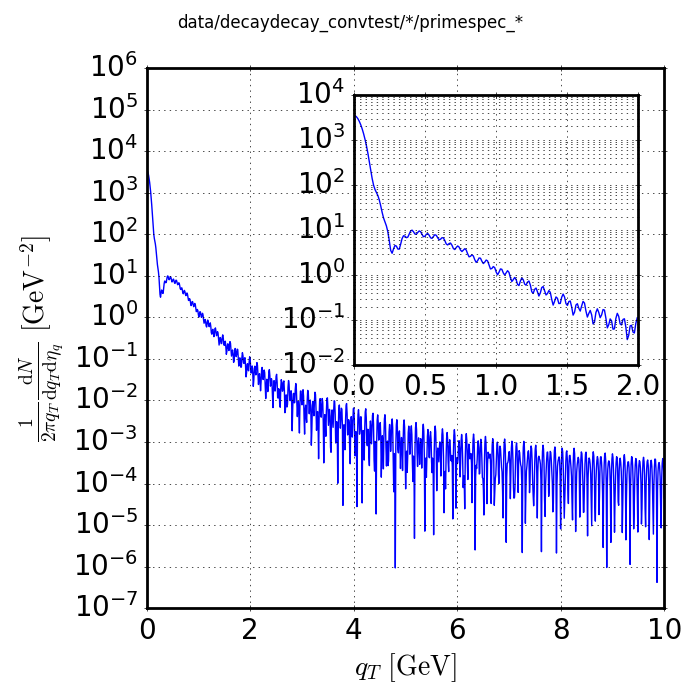
\includegraphics[width=\linewidth]{code/C++/DCCspec/images/decaydecay_convtest_primespec.png}        
            \end{minipage}
        }
        \debugbox{
            \begin{minipage}{0.45\linewidth}
                \centering
                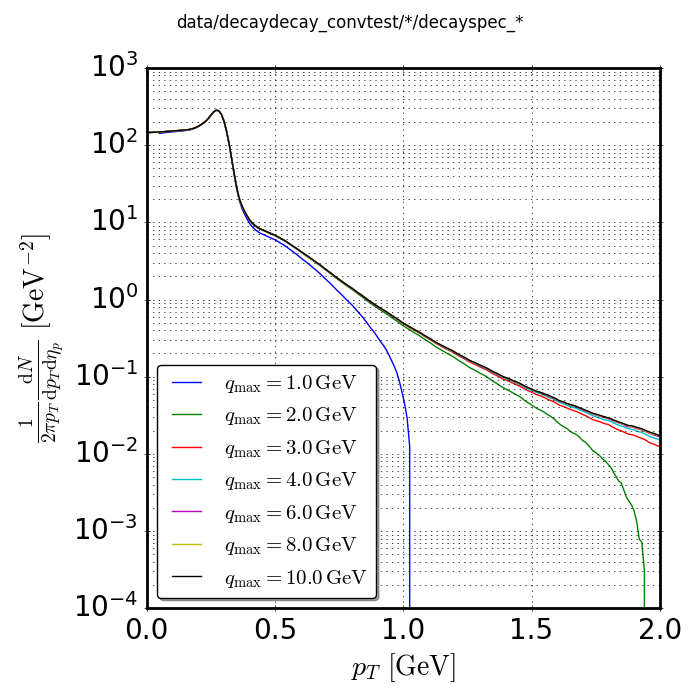
\includegraphics[width=\linewidth]{code/C++/DCCspec/images/decaydecay_convtest_decayspecs.png}        
            \end{minipage}
        }
        \captionof{figure}{Underlying spectrum of the primary heavy resonance $a$ (left) and resulting spectra of the lighter resonance $b$ (right), for different restrictions on $q_{T,\text{max}}$.}
        \label{fig:decayspec_convtest}
    \end{minipage}
}
Analyzing figure \ref{fig:decayspec_convtest}, we derive that in order to compute the decay spectrum of the lighter resonance $b$ up to transverse momenta $p_T$, on should compute the spectrum of the heavy reasonance $a$ up to ${q_T>p_T}$. The most prominent feature of the decay spectrum is a plateau in the region ${p_T\in[0,p^a_{b\vert c}]}$. Having spent thoughts on the implications of energy conversation on the details of the computation already, it is easy to give an explanation on the origin of this plateau structure. As we saw in the last chapter, all primary spectra computed here are significantly peaked around ${q_T=0\,\text{GeV}}$. Only for ${p_T< p^a_{b\vert c}}$ or ${\omega_{p,T}<E^a_{b\vert c}}$ can the primary resonance be at rest and the large peak of the pimary spectrum contributes in the decay spectrum. For larger $p_T$, energy conservation requires the primary resonance to have non-vanishing momentum ${q_T>0}$ oriented approximately parallel to the momentum of magnitude ${p_T}$ of the decay product. This is essentially the statement of figure \ref{fig:DecayCalc_IntegrDom}.

\paragraph{Sensitivity on Initial Conditions}

In chapter \ref{sec:ExampleSpectra} we systematically tested 1-parameter families of initical condition within the ${\epsilon=\const}$-prescription. Recalling the spectra presented there, noticeable differences are especially present for larger particle masses. Thus, we should also study how these differences in initial conditions affect the shape of the spectra of the decay products. The results of this investigation are shown in the following figure \ref{fig:decayspec_inittest}.\\\noindent
\debugbox{
    \begin{minipage}{\linewidth}
        \centering
        \debugbox{
            \begin{minipage}{0.45\linewidth}
                \centering
                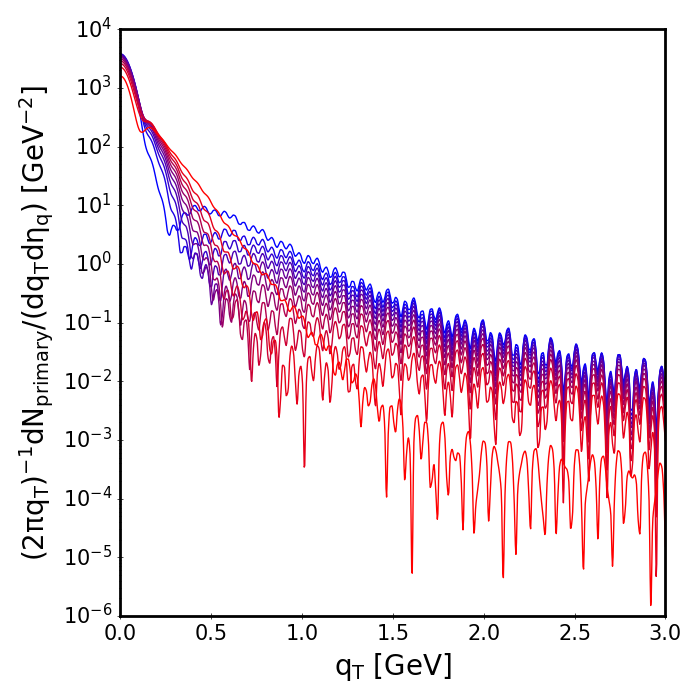
\includegraphics[width=\linewidth]{code/C++/DCCspec/images/decaydecay_inittest_primespec.png}        
            \end{minipage}
        }
        \debugbox{
            \begin{minipage}{0.45\linewidth}
                \centering
                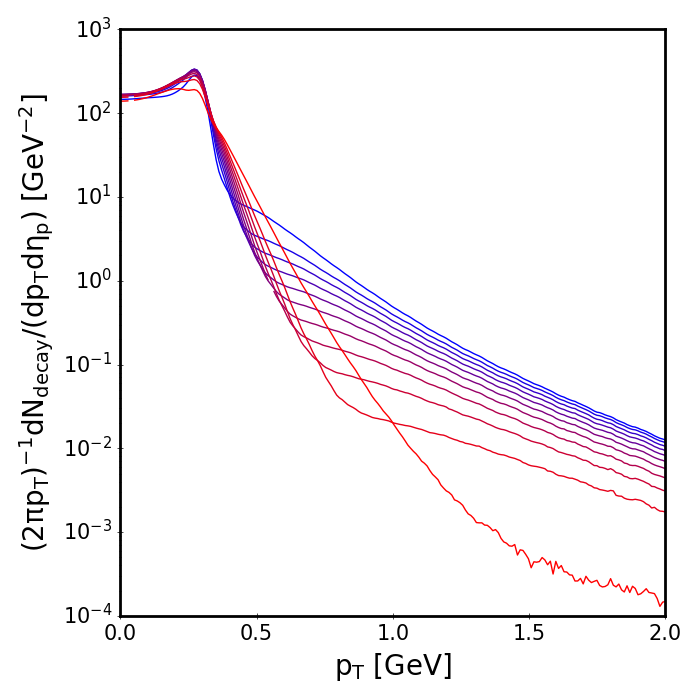
\includegraphics[width=\linewidth]{code/C++/DCCspec/images/decaydecay_inittest_decayspecs.png}        
            \end{minipage}
        }
        \captionof{figure}{Underlying spectra of the primary heavy resonance $a$ (left) and resulting spectra of the lighter resonance $b$ (right), for different initial conditions (compare e.g. figure \ref{fig:SpecRealConstEps_m570}).}
        \label{fig:decayspec_inittest}
    \end{minipage}
}
For the low $p_T$ regime of the decay spectra, especially the aforementioned ${p_T<p^a_{b\vert c}}$ plateau, the precise initial conditions of the primary resonance do not play a significant role. Differences appear only at ${p_T>p^a_{b\vert c}}$, where we expect the effects of the condensate fields on the measurement to be negligible anyways.





Let us try to evaluate the decay map in the rest frame of the decay product b, such that $p^\mu=(m_b,\vec{0})$.
\begin{subequations}
    \begin{align}
        \omega_{\vec{p}}\frac{\dt N_b}{\dt^3p}&=B\frac{4\pi^2m_a}{p^a_{b\vert c}}\times2\pi\int\frac{\dt^4q}{(2\pi)^4}\delta(q^2+m_a^2)\Big(\omega_{\vec{q}}\frac{\dt N_a}{\dt^3 q}\Big)\delta\big(q^\mu p_\mu+m_a E^a_{b\vert c}\big)\\
        &=B\frac{4\pi^2m_a}{p^a_{b\vert c}}\times2\pi\int\frac{\dt q^0\dt q^3\dt Q Q\dt\varphi}{(2\pi)^4}\delta(q^2+m_a^2)\Big(\omega_{\vec{q}}\frac{\dt N_a}{\dt^3 q}\Big)\delta\big(-m_bq^0+m_a E^a_{b\vert c}\big)\\
        &=B\frac{4\pi^2m_a}{p^a_{b\vert c}}\times\frac{2\pi}{m_b}\int\frac{\dt q^3\dt Q Q\dt\varphi}{(2\pi)^4}\delta\Big(\underbrace{-\frac{m_a^2E_{a\rightarrow b\vert c}^2}{m_b^2}+m_a^2}_{=-\frac{m_a^2p_{a\rightarrow b\vert c}^2}{m_b^2}}+(q^3)^2+Q^2\Big)\Big(\omega_{\vec{q}}\frac{\dt N_a}{\dt^3 q}\Big)\\
        \intertext{\dots define $q^3=w\frac{m_a p^a_{b\vert c}}{m_b}$\dots}
        &=B\frac{4\pi^2m_a}{p^a_{b\vert c}}\times\frac{(2\pi)^2 m_ap_{a\rightarrow b\vert c}}{m_b^2}\int\frac{\dt w\dt Q Q}{(2\pi)^4}\delta\Big(Q^2-(1-w^2)\frac{m_a^2p_{a\rightarrow b\vert c}^2}{m_b^2}\Big)\Big(\omega_{\vec{q}}\frac{\dt N_a}{\dt^3 q}\Big)\\
        &=B\frac{4\pi^2m_a}{p^a_{b\vert c}}\times\frac{(2\pi)^2 m_ap_{a\rightarrow b\vert c}}{2m_b^2}\int_{-1}^1\frac{\dt w}{(2\pi)^4}\Big(\omega_{\vec{q}}\frac{\dt N_a}{\dt^3 q}\Big)\Big\vert_{Q=q^{\perp,\star}(w)}\\
    \end{align}
\end{subequations}
where we integrated out the $\delta$-function over $Q$, using $\delta(Q^2-(q^{\perp,\star})^2)=\delta(Q\pm q^{\perp,\star})/(2\vert Q\vert)$ with 
\begin{equation}
    q^{\perp,\star}(w)=\sqrt{(1-w^2)\frac{m_a^2p_{a\rightarrow b\vert c}^2}{m_b^2}}
\end{equation}
and the condition $Q^2\geq 0$ implies $w\in[-1,1]$.

The process of interest for our scenario is the decay
\begin{equation}
    \sigma\to\pi\pi\,.
\end{equation}
We need a fixed mass of initial and final particle state in order to perform the above computation. The $\sigma$-meson however is a broad resonance, that is described very poorly by a $\delta$-peak in the mass spectrum. Starting from a free particle propagator ${\propto(p^2+m^2)^{-1}}$ in a QFT, the pole at ${p^2=-m^2}$ is modified when loop corrections induced by interactions in the theory are included,
\begin{equation}
    D_{\text{free}}(p;m)=-\frac{1}{p^2+m^2\pm\imagu\epsilon}\to D(p;M)=-\frac{1}{p^2+M^2-\imagu\Im\Pi}\,,
    \label{eq:1LoopPropCorrection_SelfEnergy}
\end{equation}
where $\Pi$ is the self energy, the real part of which is implicitly contained in the mass shift ${m^2\to M^2}$. In the Källen-Lehmann representation, the propagator is written as a weighted sum/integral over free propagators for different mass-squared parameters,
\begin{equation}
    D(p;M)=\int_0^\infty\dt\mu^2\rho(\mu^2)D_{\text{free}}(p;\mu)=-\int_0^\infty\dt\mu^2\frac{\rho(\mu^2)}{p^2+\mu^2}
\end{equation}
where
\begin{equation}
    \rho(\mu^2)=-\frac{1}{\pi}\Im D(p;M)
\end{equation}
is the spectral density. In the non-interacting limit one recovers the $\delta$-peak at ${\mu^2=m^2}$ by taking the limit ${\epsilon\to 0}$ on the left side of equation \eqref{eq:1LoopPropCorrection_SelfEnergy}. The self energy $\Pi$ can be calculated perturbatively from loop-integrals. A common approximation is given in terms of the Breit-Wigner parametrization, which assumes a momentum independent value ${\Im\Pi=M\Gamma}$. The constant $\Gamma$ is then called the Breit-Wigner width.

A resonance is typically characterized by the position of a complex pole in the scattering matrix of a given process,
\begin{equation}
    \sqrt{s_p}=M_p-\imagu\Gamma_p/2\,.
\end{equation}
For very narrow resonances, the Breit-Wigner parametrization mentioned above can be a good estimate and the peak and width of the spectral density are approximately equal to real and imaginary part of the complex pole of the propagator, ${\sqrt{s_p}\approx M-\imagu\Gamma/2}$. The approximation fails for broad resonances where the width is large compared to the distance to a production threshold. In the present example, such a threshold is given by the interaction of the $\sigma$-meson with the pions as the lightest interaction partners, and has the value of ${(\mu^2)_{\text{min}}=4m_\pi^2}$. The spectral density must vanish below this threshold, which is obviously not modelled well by the Breit-Wigner form.

A useful and simple parametrization in the proximity of thresholds, in the context of the $\sigma\pi\pi$-interaction is given in terms of the Sill parametrization \cite{GiacosaEtAl_2021}
\begin{equation}
    \rho(\mu^2)=-\Im\Big(\frac{1}{\mu^2-M^2+\imagu\tilde{\Gamma}\sqrt{\mu^2-(2m_\pi)^2}}\Big)\Theta\big(\mu^2-(2m_\pi)^2\big)\,.
\end{equation}
This distribution is normalized,
\begin{equation}
    \int_0^\infty\dt\mu^2\rho(\mu^2)=\int_0^\infty 2\mu\dt\mu\rho(\mu^2)=1\,,
\end{equation}
and we shall interprete it as a probability distribution, weighing the spectra computed from the decay ${\sigma\to\pi\pi}$ for different masses $m_\sigma=\mu$. From the pole coordinates $M_p$ and $\Gamma_p$ the corresponding parameters entering the above parametrization are
\begin{subequations}
    \begin{align}
        M&=\sqrt{\frac{16 m_\pi^2+\sqrt{16\Gamma_p^2M_p^2+(-16 m_\pi^2-\Gamma_p^2+4M_p^2)^2}}{4}}\,,\\
        \tilde{\Gamma}&=\sqrt{\frac{16 m_\pi^2+\Gamma_p^2-4 M_p^2+\sqrt{16\Gamma_p^2M_p^2+(-16 m_\pi^2-\Gamma_p^2+4M_p^2)^2}}{2}}\,,
    \end{align}
\end{subequations}
which is found by requesting ${\mu^2=s_p}$ to be the complex pole of the full propagator in the chosen parametrization.

There is an ongoing debate about the nature of the $\sigma$-meson. There are multiple resonances, e.g. $f_0(500)$, $f_0(980)$, $f_0(1370)$, etc. that share the same quantum numbers ${I^G(J^{PC})=0^+(0^{++})}$ as the quark-antiquark state ${\overline{\psi}\psi}$ that forms the isospin singlet derived from the group theoretic implications of the approximate $SU(2)$ symmetry between up- and down-quarks. In reality however, it is expected that this two-quark state mixes with other bound states, like four-quark states ("tetraquarks"), hadronic molecules or gluonic states to what is experimentally (indirectly) observed as the $\sigma$-meson. For more detail, see for example the review "Scalar Mesons below 1 GeV" within the Particle Data Booklet (PDG) \cite{Navasothers_2024}. Thus, it is a priori unclear which the correct resonance properties are. We expect the most dominant contribution to the soft pion spectra to arise from the lightest availabe resonance and thus choose the $f_0(500)$ with a pole position, derived from what is called the "most advanced dispersive analyses" \cite{Navasothers_2024} in the PDG, at
\begin{equation}
    \sqrt{s_p}=449-\imagu 275\,\text{MeV}\,.
\end{equation}


\debugbox{
    \begin{minipage}{\linewidth}
        \centering
                \centering
                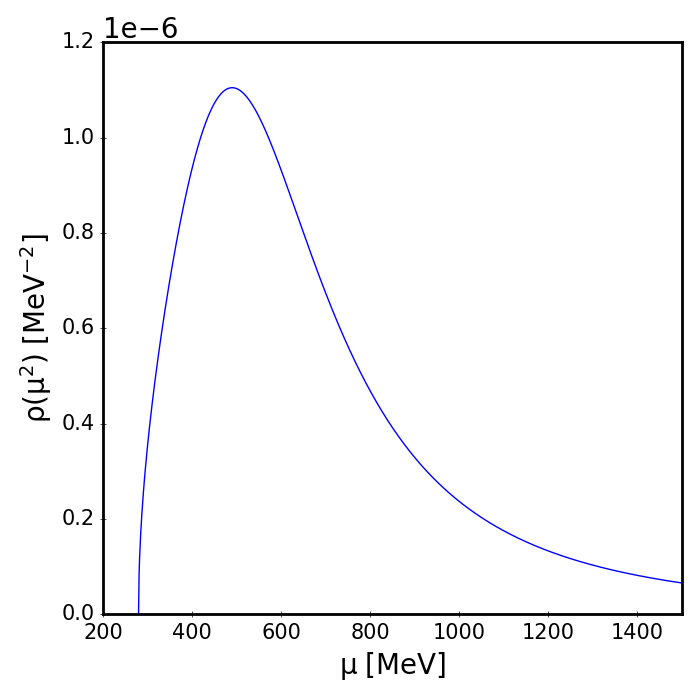
\includegraphics[width=0.6\linewidth]{code/C++/DCCspec/images/decay_sigmaresonance_pi_m140_decayspec_weights.png}
        \captionof{figure}{Spectral density function of the $\sigma$-resonance.}
        \label{fig:spectral_density_sigma}
    \end{minipage}
}